\documentclass[a4paper,12pt]{article}
\usepackage[justification=centering]{caption}
\usepackage[utf8]{inputenc}
\usepackage[T1]{fontenc}
\usepackage[romanian]{babel}
\usepackage[table]{xcolor}
\usepackage{graphicx}
\usepackage{geometry}
\usepackage{diagbox}
\usepackage{amsmath}
\usepackage{float}
\usepackage{tikz}
\usetikzlibrary{shapes, arrows, positioning, circuits.logic.US, calc, fit, backgrounds}

% Setări pagină
\geometry{margin=2.5cm}

\begin{document}

% 1. Pagina de titlu
\begin{titlepage}
    \begin{center}
        \vspace*{1cm}
        
        % Placeholder Logo
        % \begin{tikzpicture}
        %     \node[draw, minimum size=3cm, text width=2.5cm, align=center] {LOGO \\ ORGANIZAȚIE};
        % \end{tikzpicture}
        
        \vspace{1.5cm}
        
        {\Large \textbf{Universitatea Politehnica București} \par}
        \vspace{0.5cm}
        {\large Facultatea de Automatică și Calculatoare \par}
        
        \vspace{3cm}
        
        {\Huge \textbf{Implementarea unui Dispozitiv portabil de comunicații bidirecționale} \par}
        
        \vspace{0.5cm}
        {\Large Proiectare Logică - Proiect 2026 \par}
        

        \vspace{3cm}
        
        {\large \textbf{Proiect realizat de:} \par}
        \vspace{0.5cm}
        {\Large Sandu Eric-Andrei \par}
        \vspace{0.2cm}
        {\Large Mateciuc Vlad-Ștefan \par}
        \vspace{0.2cm}
        {\Large Hâncu David-Andrei \par}
        
        \vfill
        
    \end{center}
        
\end{titlepage}


\newpage
\tableofcontents
\newpage

% 2. Descrierea proiectului
\section{Descrierea funcționării automatului}
Să se proiecteze un automat secvențial sincron care controlează funcționarea unui aparat portabil de emisie-recepție (Walkie-Talkie).

Scopul automatului este de a facilita comunicarea bidirecțională între două dispozitive, permițând utilizatorului să transmită și să primească un flux audio.

Sistemul pornește într-o stare de așteptare (Idle/Listening), monitorizând semnalele de intrare. Comportamentul dispozitivului este dictat prin următoarele stări:

\begin{itemize}
    \item \textbf{Modul Normal (Receiving/Transmitting):} În starea implicită, dispozitivul primește un flux audio de la canalul său curent.
    Dacă se apasă butonul \texttt{PTT} (Push-to-Talk), automatul trece în modul de transmisie, activând microfonul și LED-ul de transmisie.
    La eliberarea butonului, revine în modul de recepție.
    
    \item \textbf{Modul Pairing:} La apăsarea butonului \texttt{PAIR}, dispozitivul intră într-o secvență de scanare, așteptând un răspuns (handshake), urmată de o stare de succes sau eroare.
    
    \item \textbf{Selectarea Canalului:} Dispozitivul permite comutarea între două canale salvate. Canalul activ este schimbat prin apăsarea \texttt{CH\_BTN}.
\end{itemize}


% 3. Schema bloc
\section{Schema bloc a automatului}
Figura \ref{fig:asm_block} prezintă intrările și ieșirile unității centrale de control. Automatul primește semnale de la interfața cu utilizatorul (butoane) și de la modulul radio (semnale de stare), generând comenzi pentru componentele hardware (LED-uri, Audio).

\begin{figure}[H]
    \centering
    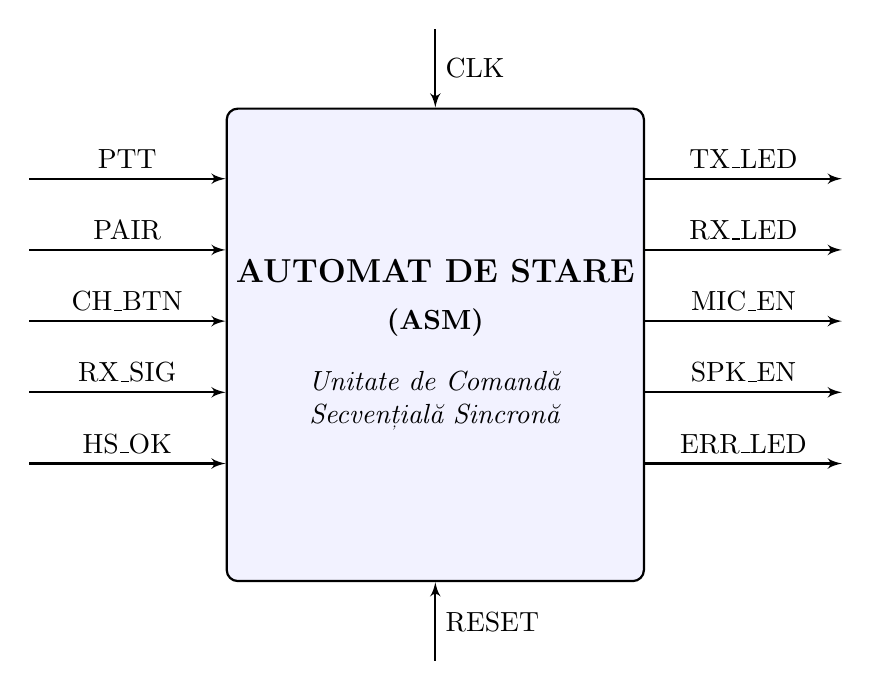
\begin{tikzpicture}[auto, node distance=1.5cm, >=latex', thick]
        % Stiluri
        \tikzstyle{block} = [draw, rectangle, minimum height=6cm, minimum width=5cm, align=center, fill=blue!5, rounded corners]
        \tikzstyle{input} = [coordinate]
        \tikzstyle{output} = [coordinate]

        % Blocul Central - Automatul
        \node [block] (asm) {
            \textbf{\large AUTOMAT DE STARE} \\[0.5em] 
            \textbf{(ASM)} \\[1em] 
            \textit{Unitate de Comandă} \\ 
            \textit{Secvențială Sincronă}
        };

        % --- INTRĂRI (Stânga) ---
        \coordinate (in_ptt) at ($(asm.north west)!0.15!(asm.south west)$);
        \coordinate (in_pair) at ($(asm.north west)!0.30!(asm.south west)$);
        \coordinate (in_ch) at ($(asm.north west)!0.45!(asm.south west)$);
        \coordinate (in_rx) at ($(asm.north west)!0.60!(asm.south west)$);
        \coordinate (in_hs) at ($(asm.north west)!0.75!(asm.south west)$);

        \draw [<-] (in_ptt) -- ++(-2.5,0) node[midway, above] {PTT};
        \draw [<-] (in_pair) -- ++(-2.5,0) node[midway, above] {PAIR};
        \draw [<-] (in_ch) -- ++(-2.5,0) node[midway, above] {CH\_BTN};
        \draw [<-] (in_rx) -- ++(-2.5,0) node[midway, above] {RX\_SIG};
        \draw [<-] (in_hs) -- ++(-2.5,0) node[midway, above] {HS\_OK};

        % --- IEȘIRI (Dreapta) ---
        \coordinate (out_tx) at ($(asm.north east)!0.15!(asm.south east)$);
        \coordinate (out_rx) at ($(asm.north east)!0.30!(asm.south east)$);
        \coordinate (out_mic) at ($(asm.north east)!0.45!(asm.south east)$);
        \coordinate (out_spk) at ($(asm.north east)!0.60!(asm.south east)$);
        \coordinate (out_err) at ($(asm.north east)!0.75!(asm.south east)$);

        \draw [->] (out_tx) -- ++(2.5,0) node[midway, above] {TX\_LED};
        \draw [->] (out_rx) -- ++(2.5,0) node[midway, above] {RX\_LED};
        \draw [->] (out_mic) -- ++(2.5,0) node[midway, above] {MIC\_EN};
        \draw [->] (out_spk) -- ++(2.5,0) node[midway, above] {SPK\_EN};
        \draw [->] (out_err) -- ++(2.5,0) node[midway, above] {ERR\_LED};

        % --- CLK și RESET ---
        \draw [<-] (asm.north) -- ++(0,1) node[midway, right] {CLK};
        \draw [<-] (asm.south) -- ++(0,-1) node[midway, right] {RESET};

    \end{tikzpicture}
    \caption{Schema bloc detaliată a automatului de stare pentru un singur dispozitiv.}
    \label{fig:asm_block}
\end{figure}

\newpage

\subsection{Descrierea Semnalelor}

Tabelul de mai jos detaliază rolul fiecărui semnal identificat în schema bloc:

\begin{description}
    \item[Intrări (Senzori și Interfață):] \hfill
    \begin{itemize}
        \item \textbf{PTT (Push-To-Talk):} Semnal activ pe '1' când utilizatorul ține apăsat butonul de vorbire. Comandă tranziția din starea de ascultare în cea de emisie.
        \item \textbf{PAIR:} Buton monostabil pentru inițierea procedurii de împerechere cu un alt dispozitiv.
        \item \textbf{CH\_BTN:} Buton pentru comutarea ciclică a canalului de comunicație (Canal 1 / Canal 2).
        \item \textbf{RX\_SIG:} Semnal digital venit de la modulul receptor radio care indică prezența unei purtătoare (carrier detect) sau a unui semnal audio valid pe canalul curent.
        \item \textbf{HS\_OK (Handshake OK):} Semnal logic generat de subsistemul de decodificare a datelor. Devine '1' doar dacă, în timpul modului de Pairing, se primește un cod corect de confirmare de la celălalt dispozitiv.
    \end{itemize}
    
    \item[Ieșiri (Comenzi Hardware):] \hfill
    \begin{itemize}
        \item \textbf{TX\_LED:} Activează LED-ul roșu pentru a indica transmisia în curs.
        \item \textbf{RX\_LED:} Activează LED-ul verde pentru a indica recepția unui semnal sau un canal liber.
        \item \textbf{MIC\_EN:} Activează preamplificatorul de microfon și modulatorul emițătorului.
        \item \textbf{SPK\_EN:} Activează amplificatorul audio final pentru difuzor (Speaker).
        \item \textbf{ERR\_LED:} LED galben/intermitent care semnalizează eșecul procesului de pairing (timeout sau lipsă handshake).
    \end{itemize}
\end{description}


\subsection{Interacțiunea în Modul Pairing}

Pentru a justifica complexitatea automatului și necesitatea stării de "Handshake" (\texttt{HS\_OK}), Figura \ref{fig:pairing_system} ilustrează interacțiunea conceptuală între două unități.

\begin{figure}[H]
    \centering
    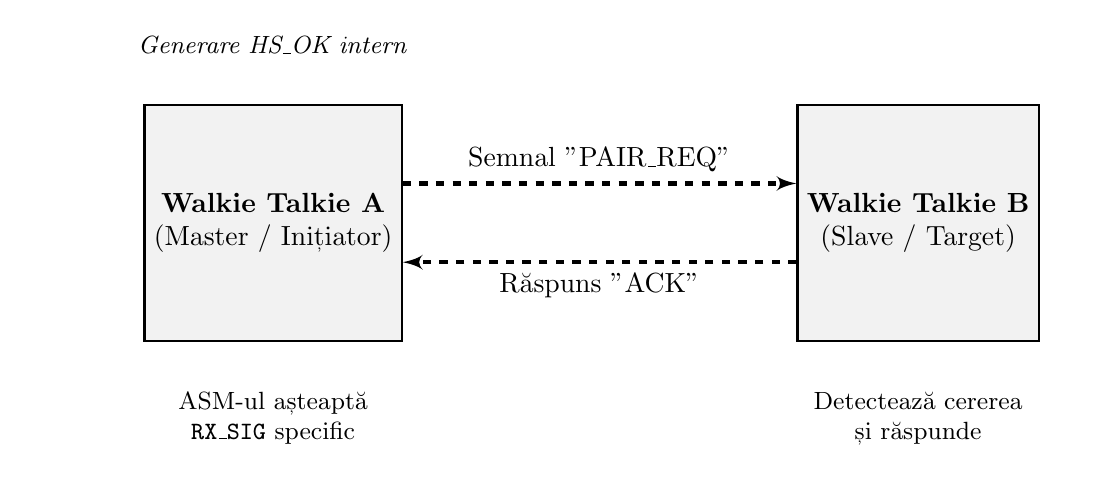
\begin{tikzpicture}[auto, node distance=3cm, >=latex', thick]
        \tikzstyle{device} = [draw, rectangle, minimum height=3cm, minimum width=2.5cm, align=center, fill=gray!10]
        
        % Dispozitiv A
        \node [device] (devA) {\textbf{Walkie Talkie A} \\ (Master / Inițiator)};
        
        % Dispozitiv B
        \node [device, right=5cm of devA] (devB) {\textbf{Walkie Talkie B} \\ (Slave / Target)};
        
        % Săgeți de comunicare RF
        \draw [->, dashed, line width=1.5pt] ($(devA.east)+(0,0.5)$) -- node[above] {Semnal "PAIR\_REQ"} ($(devB.west)+(0,0.5)$);
        \draw [->, dashed, line width=1.5pt] ($(devB.west)+(0,-0.5)$) -- node[below] {Răspuns "ACK"} ($(devA.east)+(0,-0.5)$);
        
        % Logică internă - descrieri sub dispozitive
        \node [below=0.5cm of devA, text width=4cm, align=center, font=\small] {ASM-ul așteaptă \\ \texttt{RX\_SIG} specific};
        \node [below=0.5cm of devB, text width=4cm, align=center, font=\small] {Detectează cererea \\ și răspunde};
        
        % Vizualizare generare HS_OK
        \node [above=0.5cm of devA, text width=6cm, align=center, font=\small] {\textit{Generare HS\_OK intern}};

    \end{tikzpicture}
    \caption{Schema logică a procesului de Pairing. Semnalul \texttt{HS\_OK} este generat intern de Dispozitivul A doar la recepția confirmării (ACK) de la Dispozitivul B.}
    \label{fig:pairing_system}
\end{figure}

\newpage

% 4. Organigrama
\section{Organigrama automatului}
Organigrama din Figura \ref{fig:organigram} descrie fluxul logic al automatului, evidențiind cele 5 ieșiri principale generate în stările cheie.

\begin{figure}[H]
    \centering
    \usetikzlibrary{shapes.multipart}
    
    % Stiluri
    \tikzstyle{state} = [circle, draw, minimum size=1.0cm, align=center, fill=white, font=\footnotesize\bfseries, inner sep=0pt]
    \tikzstyle{moore} = [circle split, draw, minimum size=1.1cm, align=center, fill=cyan!15, font=\footnotesize\bfseries, inner sep=1pt]
    \tikzstyle{decision} = [diamond, draw, aspect=2.5, inner sep=0pt, minimum width=2.0cm, align=center, fill=yellow!15, font=\scriptsize]

    \begin{tikzpicture}[->, >=latex', shorten >=1pt, auto, node distance=2cm, semithick, font=\footnotesize]

        % --- COLOANA CENTRALĂ ---
        \node[state] (S0) {S0\\IDLE};
        \node[decision, below=1.5cm of S0] (d_pair) {PAIR};
        \node[decision, below=1.5cm of d_pair] (d_ch) {CH\_BTN};
        \node[state, below=1.5cm of d_ch] (S10) {S10\\WAIT};
        \node[decision, below=1.5cm of S10] (d_rx) {RX\_SIG};
        \node[decision, below=1.5cm of d_rx] (d_ptt) {PTT};

        % --- RAMURA STÂNGA (Pairing) ---
        \node[state, left=4.2cm of d_pair] (S1) {S1\\INIT};
        \node[state, below=1cm of S1] (S2) {S2\\SCAN};
        \node[decision, below=1cm of S2] (d_found) {RX\_SIG};
        \node[state, left=1.5cm of d_found] (S3) {S3\\RETRY};
        \node[state, below=1cm of d_found] (S4) {S4\\SHAKE};
        \node[decision, below=1cm of S4] (d_hs) {HS\_OK};
        \node[moore, below left=1.5cm and 0.5cm of d_hs] (S7) {S7\\ERR \nodepart{lower} \rule{0pt}{2.5ex}\scriptsize ERR\_LED};
        \node[state, below right=1.5cm and 0.5cm of d_hs] (S5) {S5\\SAVE};
        \node[state, below=1cm of S5] (S6) {S6\\SUCC};

        % --- RAMURA DREAPTA (Channel & RX) ---
        \node[state, right=2.8cm of d_ch] (S8) {S8\\CH1};
        \node[state, below=0.7cm of S8] (S9) {S9\\CH2};
        \node[moore, right=2.0cm of d_rx] (S11) {S11\\LSTN \nodepart{lower} \rule{0pt}{2.5ex}\scriptsize SPK\_EN\\\scriptsize RX\_LED};

        % --- RAMURA JOS (Transmisie) ---
        \node[state, below left=1.5cm and 0.5cm of d_ptt] (S12) {S12\\PRE\_TX};
        \node[moore, below=1cm of S12] (S13) {S13\\TRSM \nodepart{lower} \rule{0pt}{2.5ex}\scriptsize MIC\_EN\\\scriptsize TX\_LED};
        \node[decision, right=1.2cm of S13] (d_rel) {PTT};
        \node[state, above=1cm of d_rel] (S14) {S14\\POST};
        \node[state, right=1.0cm of S14] (S15) {S15\\LOG};

        % --- CONEXIUNI ---
        \path (S0) edge (d_pair);
        \path (d_pair) edge node[above] {1} (S1);
        \path (S1) edge (S2);
        \path (S2) edge (d_found);
        
        % Scan Logic
        \path (d_found) edge node[above] {0} (S3);
        \path (S3) |- ([yshift=0.2cm]S2.west) -- (S2.west);
        \path (S3) edge (d_found);
        \path (d_found) edge node[right] {1} (S4);
        \path (S4) edge (d_hs);
        
        % Handshake Logic
        \draw [->] (d_hs.west) -| node[near start, above] {0} (S7.north);
        \draw [->] (d_hs.east) -| node[near start, above] {1} (S5.north);
        \path (S5) edge (S6);

        % Idle -> Channel
        \path (d_pair) edge node[right] {0} (d_ch);
        \path (d_ch) edge node[above] {1} node[below, pos=0.575, font=\scriptsize, align=center] {(din CH2)} (S8);
        \draw [->] (d_ch.east) -- ++(0.8,0) |- node[pos=0.7, below, font=\scriptsize] {(din CH1)} (S9.west);
        \draw [->] (S8.east) -- ++(0.5,0) |- (S10);
        \draw (S9) |- (S10);
        \path (d_ch) edge node[right] {0} (S10);
        \path (S10) edge (d_rx);
        \path (d_rx) edge node[above] {1} (S11);
        \draw [->] (S11.north) |- ([yshift=0.3cm]S11.north) -| ([xshift=0.5cm]S10.east) -- (S10.east);

        % Wait -> TX Logic
        \path (d_rx) edge node[right] {0} (d_ptt);
        \path (d_ptt) edge node[left] {1} (S12);
        \path (S12) edge (S13);
        \path (S13) edge (d_rel);
        \path (d_rel) edge node[below] {1} (S13);
        \path (d_rel) edge node[right] {0} (S14);
        \path (S14) edge (S15);

        % --- AUTOSTRĂZI DE ÎNTOARCERE ---
        \draw [dashed, rounded corners] (d_ptt.east) -- node[above] {0} ++(4.75, 0) coordinate(lane_right) |- (S0.east);
        \draw [dashed, rounded corners] (S7.west) -- ++(-1.5, 0) coordinate(lane_left) |- (S0.west);
        \draw [dashed, rounded corners] (S6.south) -- ++(0, -0.7) -| (lane_left);
        \draw [dashed, rounded corners] (S15.east) -- ++(1, 0) -| (lane_right);

    \end{tikzpicture}
    \caption{Organigrama de tip Moore a dispozitivului de comunicații}
    \label{fig:organigram}
\end{figure}

\subsection{Descrierea detaliată a stărilor automatului}

\begin{description}
    \item[\textbf{S0 (IDLE)}] \hfill \\
    Este starea de repaus și punctul central de decizie. Aici sistemul monitorizează intrările (\texttt{PAIR}, \texttt{CH\_BTN}, \texttt{RX\_SIG}, \texttt{PTT}) pentru a determina modul de operare.

    \item[\textbf{Ramura de Pairing (S1 - S7)}] \hfill \\
    Această secvență este inițiată la apăsarea butonului \texttt{PAIR}:
    \begin{itemize}
        \item \textbf{S1 (INIT):} Inițializează variabilele necesare protocolului de împerechere.
        \item \textbf{S2 (SCAN) și S3 (RETRY):} Dispozitivul scanează frecvențele căutând un semnal; dacă nu este găsit, trece prin \texttt{RETRY} și reia scanarea.
        \item \textbf{S4 (SHAKE):} Odată detectat un semnal, se așteaptă confirmarea protocolului (Handshake - \texttt{HS\_OK}).
        \item \textbf{S7 (ERR):} Stare de eroare (tip Moore). Se activează dacă handshake-ul eșuează, generând semnalul \texttt{ERR\_LED}.
        \item \textbf{S5 (SAVE) și S6 (SUCC):} Dacă handshake-ul este valid, datele sunt salvate, iar împerecherea este marcată ca reușită.
    \end{itemize}

    \item[\textbf{Ramura de Selectare Canal (S8 - S9)}] \hfill \\
    Accesată prin apăsarea \texttt{CH\_BTN} pentru a comuta frecvența activă:
    \begin{itemize}
        \item \textbf{S8 (CH1) și S9 (CH2):} Reprezintă cele două canale disponibile. Trecerea prin aceste stări actualizează canalul activ.
    \end{itemize}

    \item[\textbf{Monitorizare și Recepție (S10 - S11)}] \hfill \\
    Gestionează traficul audio de intrare:
    \begin{itemize}
        \item \textbf{S10 (WAIT):} Stare intermediară care verifică prezența semnalului radio sau comanda de transmisie.
        \item \textbf{S11 (LSTN):} Stare activă de recepție (tip Moore). Când \texttt{RX\_SIG} este detectat, automatul activează ieșirile \texttt{SPK\_EN} (difuzor) și \texttt{RX\_LED} (indicator vizual).
    \end{itemize}

    \item[\textbf{Ramura de Transmisie (S12 - S15)}] \hfill \\
    Activată prin menținerea apăsată a butonului \texttt{PTT}:
    \begin{itemize}
        \item \textbf{S12 (PRE\_TX):} Pregătește circuitele de emisie.
        \item \textbf{S13 (TRSM):} Stare activă de transmisie (tip Moore). Menține active ieșirile \texttt{MIC\_EN} (microfon) și \texttt{TX\_LED} atâta timp cât \texttt{PTT} este apăsat.
        \item \textbf{S14 (POST) și S15 (LOG):} După eliberarea butonului, se execută operațiuni post-transmisie și logarea evenimentului înainte de revenirea în \texttt{IDLE}.
    \end{itemize}
\end{description}

\newpage

% % 5. Ecuațiile de stare
\section{Identificarea ecuațiilor de stare}
Pentru a transpune organigrama într-un circuit digital secvențial, fiecărei stări i s-a alocat un cod binar unic pe 4 biți: $Q_3 Q_2 Q_1 Q_0$.

\subsection{Codificarea Stărilor}

\begin{table}[H]
    \centering
    \begin{tabular}{|l|c|c|}
        \hline
        \textbf{Stare} & \textbf{Simbol} & \textbf{Cod ($Q_3 Q_2 Q_1 Q_0$)} \\
        \hline
        S0 & IDLE & 0000 \\
        \hline
        S1 & INIT & 0001 \\
        \hline
        S2 & SCAN & 0010 \\
        \hline
        S3 & RETRY & 0011 \\
        \hline
        S4 & SHAKE & 0100 \\
        \hline
        S5 & SAVE & 0101 \\
        \hline
        S6 & SUCC & 0110 \\
        \hline
        S7 & ERR & 0111 \\
        \hline
        S8 & CH1 & 1000 \\
        \hline
        S9 & CH2 & 1001 \\
        \hline
        S10 & WAIT & 1010 \\
        \hline
        S11 & LSTN & 1011 \\
        \hline
        S12 & PRE\_TX & 1100 \\
        \hline
        S13 & TRSM & 1101 \\
        \hline
        S14 & POST & 1110 \\
        \hline
        S15 & LOG & 1111 \\
        \hline
    \end{tabular}
    \caption{Tabela de alocare a stărilor}
\end{table}

\subsection{Definirea Variabilelor de Intrare}

Ecuațiile de tranziție depind de starea curentă și de intrările asincrone. Pentru simplificarea tabelelor, vom folosi următoarele notații:

\begin{itemize}
    \item $P$ = Buton \texttt{PAIR}
    \item $C$ = Buton \texttt{CH\_BTN}
    \item $R$ = Semnal \texttt{RX\_SIG}
    \item $H$ = Semnal \texttt{HS\_OK}
    \item $T$ = Buton \texttt{PTT}
\end{itemize}

\subsection{Hărțile Karnaugh pentru Funcția de Stare Următoare}

Vom determina funcțiile logice $Q_3^+, Q_2^+, Q_1^+, Q_0^+$ completând hărțile Karnaugh. Celulele conțin condiția logică (intrare) necesară pentru ca bitul respectiv să devină '1' în starea următoare.

% --- HARTĂ PENTRU Q3 ---
\subsubsection*{Ecuația pentru $Q_3$}

\begin{table}[H]
    \centering
    \renewcommand{\arraystretch}{1.5}
    \begin{tabular}{|c|c|c|c|c|}
        \hline
        \rowcolor{gray!20}
        \diagbox{$Q_1 Q_0$}{$Q_3 Q_2$} & \textbf{00} & \textbf{01} & \textbf{11} & \textbf{10} \\ \hline
        \textbf{00} & $\bar{P}$ & $H$ & $1$ & $1$ \\ \hline 
        \textbf{01} & $0$ & $1$ & $T$ & $1$ \\ \hline
        \textbf{11} & $0$ & $0$ & $0$ & $1$ \\ \hline
        \textbf{10} & $0$ & $0$ & $1$ & $R + \bar{R}T$ \\ \hline
    \end{tabular}
    \caption{Harta K pentru $Q_3^+$}
\end{table}

Ecuația minimizată extrasă din hartă:
\begin{equation}
\begin{split}
    Q_3^+ = & \underbrace{\overline{Q_3}\overline{Q_2}\overline{Q_1}\overline{Q_0} \cdot \bar{P}}_{S0 \to S8/10} + \underbrace{\overline{Q_3}Q_2\overline{Q_1}\overline{Q_0} \cdot H}_{S4 \to S5} + \underbrace{\overline{Q_3}Q_2\overline{Q_1}Q_0}_{S5 \to S6} \\
    & + \underbrace{Q_3\overline{Q_2}(\overline{Q_1} + Q_1Q_0 + Q_1\overline{Q_0}(R + \bar{R}T))}_{Hold\ S8, S9, S11\ \&\ S10 \to Next} \\
    & + \underbrace{Q_3Q_2(\overline{Q_1}\overline{Q_0} + \overline{Q_1}Q_0 T + Q_1\overline{Q_0})}_{S12 \to S13,\ Hold\ S13,\ S14 \to S15}
\end{split}
\end{equation}

% --- HARTĂ PENTRU Q2 ---
\subsubsection*{Ecuația pentru $Q_2$}

\begin{table}[H]
    \centering
    \renewcommand{\arraystretch}{1.5}
    \begin{tabular}{|c|c|c|c|c|}
        \hline
        \rowcolor{gray!20}
        \diagbox{$Q_1 Q_0$}{$Q_3 Q_2$} & \textbf{00} & \textbf{01} & \textbf{11} & \textbf{10} \\ \hline
        \textbf{00} & $0$ & $H$ & $1$ & $0$ \\ \hline
        \textbf{01} & $0$ & $1$ & $T$ & $0$ \\ \hline
        \textbf{11} & $0$ & $0$ & $0$ & $0$ \\ \hline
        \textbf{10} & $R$ & $0$ & $1$ & $\bar{R}T$ \\ \hline
    \end{tabular}
    \caption{Harta K pentru $Q_2^+$}
\end{table}

Ecuația minimizată extrasă din hartă:
\begin{equation}
\begin{split}
    Q_2^+ = & \underbrace{\overline{Q_3}\overline{Q_2}Q_1\overline{Q_0} \cdot R}_{S2 \to S4} + \underbrace{\overline{Q_3}Q_2\overline{Q_1}\overline{Q_0} \cdot H}_{S4 \to S5} + \underbrace{\overline{Q_3}Q_2\overline{Q_1}Q_0}_{S5 \to S6} \\
    & + \underbrace{Q_3\overline{Q_2}Q_1\overline{Q_0} \cdot \bar{R}T}_{S10 \to S12} + \underbrace{Q_3Q_2(\overline{Q_1}\overline{Q_0} + Q_1\overline{Q_0} + \overline{Q_1}Q_0 T)}_{S12, S13, S14 \text{ Logic}}
\end{split}
\end{equation}

% --- HARTĂ PENTRU Q1 ---
\subsubsection*{Ecuația pentru $Q_1$}

\begin{table}[H]
    \centering
    \renewcommand{\arraystretch}{1.5}
    \begin{tabular}{|c|c|c|c|c|}
        \hline
        \rowcolor{gray!20}
        \diagbox{$Q_1 Q_0$}{$Q_3 Q_2$} & \textbf{00} & \textbf{01} & \textbf{11} & \textbf{10} \\ \hline
        \textbf{00} & $\bar{P}\bar{C}$ & $\bar{H}$ & $0$ & $1$ \\ \hline
        \textbf{01} & $1$ & $1$ & $\bar{T}$ & $1$ \\ \hline
        \textbf{11} & $1$ & $0$ & $0$ & $1$ \\ \hline
        \textbf{10} & $\bar{R}$ & $0$ & $1$ & $R$ \\ \hline
    \end{tabular}
    \caption{Harta K pentru $Q_1^+$}
\end{table}

Ecuația minimizată extrasă din hartă:
\begin{equation}
\begin{split}
    Q_1^+ = & \underbrace{\overline{Q_3}\overline{Q_2}\overline{Q_1}\overline{Q_0} \cdot \bar{P}\bar{C}}_{S0 \to S10} + \underbrace{\overline{Q_3}\overline{Q_2}(\overline{Q_1}Q_0 + Q_1Q_0 + Q_1\overline{Q_0}\bar{R})}_{S1 \to S2,\ S3 \to S2,\ S2 \to S3} \\
    & + \underbrace{\overline{Q_3}Q_2\overline{Q_1}\overline{Q_0} \cdot \bar{H}}_{S4 \to S7} + \underbrace{\overline{Q_3}Q_2\overline{Q_1}Q_0}_{S5 \to S6} \\
    & + \underbrace{Q_3\overline{Q_2}(\overline{Q_1}\overline{Q_0} + \overline{Q_1}Q_0 + Q_1Q_0 + Q_1\overline{Q_0}R)}_{Channel\ Logic\ \&\ S10 \to S11} \\
    & + \underbrace{Q_3Q_2\overline{Q_1}Q_0 \cdot \bar{T}}_{S13 \to S14} + \underbrace{Q_3Q_2Q_1\overline{Q_0}}_{S14 \to S15}
\end{split}
\end{equation}

% --- HARTĂ PENTRU Q0 ---
\subsubsection*{Ecuația pentru $Q_0$}

\begin{table}[H]
    \centering
    \renewcommand{\arraystretch}{1.5}
    \begin{tabular}{|c|c|c|c|c|}
        \hline
        \rowcolor{gray!20}
        \diagbox{$Q_1 Q_0$}{$Q_3 Q_2$} & \textbf{00} & \textbf{01} & \textbf{11} & \textbf{10} \\ \hline
        \textbf{00} & $P$ & $H$ & $1$ & $C$ \\ \hline
        \textbf{01} & $0$ & $0$ & $T$ & $0$ \\ \hline
        \textbf{11} & $0$ & $0$ & $0$ & $0$ \\ \hline
        \textbf{10} & $\bar{R}$ & $0$ & $0$ & $R$ \\ \hline
    \end{tabular}
    \caption{Harta K pentru $Q_0^+$}
\end{table}

Ecuația minimizată extrasă din hartă:
\begin{equation}
\begin{split}
    Q_0^+ = & \underbrace{\overline{Q_3}\overline{Q_2}\overline{Q_1}\overline{Q_0} \cdot P}_{S0 \to S1} + \underbrace{\overline{Q_3}\overline{Q_2}Q_1\overline{Q_0} \cdot \bar{R}}_{S2 \to S3} + \underbrace{\overline{Q_3}Q_2\overline{Q_1}\overline{Q_0} \cdot H}_{S4 \to S5} \\
    & + \underbrace{Q_3\overline{Q_2}\overline{Q_1}\overline{Q_0} \cdot C}_{S8 \to S9} + \underbrace{Q_3\overline{Q_2}Q_1\overline{Q_0} \cdot R}_{S10 \to S11} \\
    & + \underbrace{Q_3Q_2(\overline{Q_1}\overline{Q_0} + Q_1\overline{Q_0} + \overline{Q_1}Q_0 T)}_{S12 \to S13, S14 \to S15, Hold\ S13}
\end{split}
\end{equation}

\newpage

% 6. Implementare CBB + MUX
\section{Implementarea cu CBB JK și Multiplexoare 4:1}
% ==================================================
% DEFINIȚII STILURI GLOBALE (TIKZ)
% ==================================================
\tikzset{
    % Stil MUX: Text centrat, în interior
    mux/.style={
        draw, rectangle, minimum width=2.0cm, minimum height=3.5cm, thick, fill=white, 
        align=center, font=\small\bfseries
    },
    % Stil CBB: Text centrat, în interior
    cbb/.style={
        draw, rectangle, minimum width=2.5cm, minimum height=2.5cm, thick, fill=white, 
        align=center, font=\bfseries
    },
    wire/.style={thick, ->, >=latex},
    % Stil pentru eticheta binară (00, 01...): La stânga pinului, font mic
    binlbl/.style={font=\tiny, anchor=east, xshift=-1pt, inner sep=1pt}
}
\newcommand{\tablestretch}{1.4}
\newcommand{\tablefontsize}{\footnotesize}

% --- Q3 ---
\subsection{Implementarea etajului $Q_3$}
\textbf{Selectori:} $Q_1, Q_0$ (Liniile hărții). Logica intrărilor $D_i$ depinde de $Q_2$ (Coloane).

\begin{figure}[H]
    \centering
    \begin{tikzpicture}[font=\footnotesize]
        % --- TABELE SIDE-BY-SIDE ---
        % Tabel J (Stânga)
        \node (tableJ) at (0,0) [anchor=north west] {
            \renewcommand{\arraystretch}{\tablestretch}
            \tablefontsize
            \begin{tabular}{|c|c|c|}
                \hline
                \rowcolor{green!20}
                \diagbox[width=2.2cm]{$Q_1 Q_0$}{$Q_3 Q_2$} & \textbf{00} & \textbf{01} \\ \hline
                \textbf{00} ($D_0$) & $\bar{P}$ & $0$ \\ \hline
                \textbf{01} ($D_1$) & $0$ & $0$ \\ \hline
                \textbf{11} ($D_3$) & $0$ & $0$ \\ \hline
                \textbf{10} ($D_2$) & $0$ & $0$ \\ \hline
            \end{tabular}
        };
        \node[above, green!50!black] at (tableJ.north) {\textbf{Zona J ($Q_3=0$)}};

        % Tabel K (Dreapta - Spațiat)
        \node (tableK) at (7.5,0) [anchor=north west] {
            \renewcommand{\arraystretch}{\tablestretch}
            \tablefontsize
            \begin{tabular}{|c|c|c|}
                \hline
                \rowcolor{red!20}
                \diagbox[width=2.2cm]{$Q_1 Q_0$}{$Q_3 Q_2$} & \textbf{11} & \textbf{10} \\ \hline
                \textbf{00} ($D_0$) & $0$ & $0$ \\ \hline
                \textbf{01} ($D_1$) & $0$ & $0$ \\ \hline
                \textbf{11} ($D_3$) & $1$ & $0$ \\ \hline
                \textbf{10} ($D_2$) & $0$ & $\bar{R}\bar{T}$ \\ \hline
            \end{tabular}
        };
        \node[above, red!50!black] at (tableK.north) {\textbf{Zona K ($Q_3=1$)}};

        % --- SCHEMA LOGICĂ ---
        \def\topY{-6.0}     
        \def\botY{-10.5}    
        \def\midY{-8.25}    
        \def\muxX{3.0}
        \def\cbbX{10.0}
        \def\pinOffset{0.6}

        % Componente cu Text ÎNĂUNTRU
        \node[mux] (muxJ) at (\muxX, \topY) {MUX-J\\4:1};
        \node[mux] (muxK) at (\muxX, \botY) {MUX-K\\4:1};
        \node[cbb] (jk) at (\cbbX, \midY) {CBB JK};

        % Conexiuni MUX -> CBB (90 grade)
        \draw[wire] (muxJ.east) -- ++(1.5,0) |- ($(jk.west)+(0,\pinOffset)$) node[pos=0.7, above] {$J_3$};
        \draw[wire] (muxK.east) -- ++(1.5,0) |- ($(jk.west)+(0,-\pinOffset)$) node[pos=0.7, above] {$K_3$};

        % Intrări MUX J
        \def\muxPinSpacing{0.65}
        \foreach \i/\lbl/\val in {
          1.5/00/$\overline{Q_2} \cdot \bar{P}$,
            0.5/01/$0$,
            -0.5/10/$0$,
            -1.5/11/$0$
        } {
            % Linia se desenează spre stânga (-0.8). Eticheta este pusă la mijloc (midway) și deasupra (above).
            \draw (muxJ.west) ++(0, \i*\muxPinSpacing) -- node[midway, above, font=\tiny, inner sep=1pt] {\lbl} ++(-0.8, 0) coordinate(startline);
            \node[left, align=right] at (startline) {\small \val};
        }

        % Intrări MUX K
        \foreach \i/\lbl/\val in {
            1.5/00/$0$,
            0.5/01/$0$,
            -0.5/10/$\overline{Q_2} \cdot \bar{R}\bar{T}$,
            -1.5/11/$Q_2$
        } {
            \draw (muxK.west) ++(0, \i*\muxPinSpacing) -- node[midway, above, font=\tiny, inner sep=1pt] {\lbl} ++(-0.8, 0) coordinate(startline);
            \node[left, align=right] at (startline) {\small \val};
        }
        
        % Ieșiri CBB
        \draw[wire] ($(jk.east)+(0,0.5)$) -- ++(1,0) node[right] {$Q_3$};
        \draw[wire] ($(jk.east)+(0,-0.5)$) -- ++(1,0) node[right] {$\overline{Q_3}$};

        % Selectori
        \draw[thick] (muxJ.south) -- (muxK.north);
        \draw[thick, <-] (muxK.south) -- ++(0, -0.5) node[below] {$Q_1, Q_0$};

    \end{tikzpicture}
    \caption{Implementarea grafică a etajului $Q_3$}
\end{figure}

\newpage

% --- Q2 ---
\subsection{Implementarea etajului $Q_2$}
\textbf{Selectori:} $Q_1, Q_0$ (Liniile hărții). Logica intrărilor $D_i$ depinde de $Q_3$ (Coloane).

\begin{figure}[H]
    \centering
    \begin{tikzpicture}[font=\footnotesize]
        % Tabel J
        \node (tableJ) at (0,0) [anchor=north west] {
            \renewcommand{\arraystretch}{\tablestretch}
            \tablefontsize
            \begin{tabular}{|c|c|c|}
                \hline
                \rowcolor{green!20}
                \diagbox[width=2.2cm]{$Q_1 Q_0$}{$Q_3 Q_2$} & \textbf{00} & \textbf{10} \\ \hline
                \textbf{00} ($D_0$) & $0$ & $0$ \\ \hline
                \textbf{01} ($D_1$) & $0$ & $0$ \\ \hline
                \textbf{11} ($D_3$) & $R$ & $0$ \\ \hline
                \textbf{10} ($D_2$) & $R$ & $\bar{R}T$ \\ \hline
            \end{tabular}
        };
        \node[above, green!50!black] at (tableJ.north) {\textbf{Zona J ($Q_2=0$)}};

        % Tabel K
        \node (tableK) at (7.5,0) [anchor=north west] {
            \renewcommand{\arraystretch}{\tablestretch}
            \tablefontsize
            \begin{tabular}{|c|c|c|}
                \hline
                \rowcolor{red!20}
                \diagbox[width=2.2cm]{$Q_1 Q_0$}{$Q_3 Q_2$} & \textbf{01} & \textbf{11} \\ \hline
                \textbf{00} ($D_0$) & $0$ & $0$ \\ \hline
                \textbf{01} ($D_1$) & $0$ & $0$ \\ \hline
                \textbf{11} ($D_3$) & $1$ & $1$ \\ \hline
                \textbf{10} ($D_2$) & $1$ & $0$ \\ \hline
            \end{tabular}
        };
        \node[above, red!50!black] at (tableK.north) {\textbf{Zona K ($Q_2=1$)}};

        % Parametri
        \def\topY{-6.0} \def\botY{-10.5} \def\midY{-8.25}
        \def\muxX{3.0} \def\cbbX{10.0} \def\pinOffset{0.6} \def\muxPinSpacing{0.65}

        % Componente
        \node[mux] (muxJ) at (\muxX, \topY) {MUX-J\\4:1};
        \node[mux] (muxK) at (\muxX, \botY) {MUX-K\\4:1};
        \node[cbb] (jk) at (\cbbX, \midY) {CBB JK};

        % Conexiuni
        \draw[wire] (muxJ.east) -- ++(1.5,0) |- ($(jk.west)+(0,\pinOffset)$) node[pos=0.7, above] {$J_2$};
        \draw[wire] (muxK.east) -- ++(1.5,0) |- ($(jk.west)+(0,-\pinOffset)$) node[pos=0.7, above] {$K_2$};

        % Intrări
        \foreach \i/\lbl/\val in {
            1.5/00/$0$,
            0.5/01/$0$,
            -0.5/10/$\overline{Q_3} \cdot R + Q_3 \cdot \bar{R}T$,
            -1.5/11/$\overline{Q_3} \cdot R$
        } {
            \draw (muxJ.west) ++(0, \i*\muxPinSpacing) -- node[midway, above, font=\tiny, inner sep=1pt] {\lbl} ++(-0.8, 0) coordinate(startline);
            \node[left, align=right] at (startline) {\small \val};
        }
        \foreach \i/\lbl/\val in {
            1.5/00/$0$,
            0.5/01/$0$,
            -0.5/10/$\overline{Q_3}$,
            -1.5/11/$1$
        } {
            \draw (muxK.west) ++(0, \i*\muxPinSpacing) -- node[midway, above, font=\tiny, inner sep=1pt] {\lbl} ++(-0.8, 0) coordinate(startline);
            \node[left, align=right] at (startline) {\small \val};
        }

        \draw[wire] ($(jk.east)+(0,0.5)$) -- ++(1,0) node[right] {$Q_2$};
        \draw[wire] ($(jk.east)+(0,-0.5)$) -- ++(1,0) node[right] {$\overline{Q_2}$};
        \draw[thick] (muxJ.south) -- (muxK.north);
        \draw[thick, <-] (muxK.south) -- ++(0, -0.5) node[below] {$Q_1, Q_0$};
    \end{tikzpicture}
    \caption{Implementarea grafică a etajului $Q_2$}
\end{figure}

\newpage

% --- Q1 ---
\subsection{Implementarea etajului $Q_1$}
\textbf{Selectori:} $Q_3, Q_2$ (Coloanele hărții). Logica intrărilor $D_i$ depinde de $Q_0$ (Linii).

\begin{figure}[H]
    \centering
    \begin{tikzpicture}[font=\footnotesize]
        % --- TABELE SIDE-BY-SIDE (Late) ---
        % Tabel J (Stânga)
        \node (tableJ) at (0,0) [anchor=north west] {
            \renewcommand{\arraystretch}{\tablestretch}
            \tablefontsize
            \setlength{\tabcolsep}{3pt}
            \begin{tabular}{|c|c|c|c|c|}
                \hline
                \rowcolor{green!20}
                \diagbox[width=2.4cm]{$Q_1 Q_0$}{$Q_3 Q_2$} & \textbf{00} & \textbf{01} & \textbf{11} & \textbf{10} \\ \hline
                \textbf{00} & $\bar{P}\bar{C}$ & $\bar{H}$ & $0$ & $1$ \\ \hline
                \textbf{01} & $1$ & $1$ & $\bar{T}$ & $1$ \\ \hline
            \end{tabular}
        };
        \node[above, green!50!black] at (tableJ.north) {\textbf{Zona J ($Q_1=0$)}};

        % Tabel K (Dreapta - Lângă J)
        % Ajustat poziția X la 8.2 pentru a face loc tabelelor mai mari
        \node (tableK) at (8.2,0) [anchor=north west] {
            \renewcommand{\arraystretch}{\tablestretch}
            \tablefontsize
            \setlength{\tabcolsep}{3pt}
            % MĂRIT WIDTH la 2.4cm
            \begin{tabular}{|c|c|c|c|c|}
                \hline
                \rowcolor{red!20}
                \diagbox[width=2.4cm]{$Q_1 Q_0$}{$Q_3 Q_2$} & \textbf{00} & \textbf{01} & \textbf{11} & \textbf{10} \\ \hline
                \textbf{11} & $R$ & $1$ & $1$ & $0$ \\ \hline
                \textbf{10} & $R$ & $1$ & $0$ & $\bar{R}$ \\ \hline
            \end{tabular}
        };
        \node[above, red!50!black] at (tableK.north) {\textbf{Zona K ($Q_1=1$)}};

        % Parametri
        \def\topY{-6.0} \def\botY{-10.5} \def\midY{-8.25}
        \def\muxX{3.5} \def\cbbX{10.5} \def\pinOffset{0.6} \def\muxPinSpacing{0.65}

        % Componente
        \node[mux] (muxJ) at (\muxX, \topY) {MUX-J\\4:1};
        \node[mux] (muxK) at (\muxX, \botY) {MUX-K\\4:1};
        \node[cbb] (jk) at (\cbbX, \midY) {CBB JK};

        % Conexiuni
        \draw[wire] (muxJ.east) -- ++(1.5,0) |- ($(jk.west)+(0,\pinOffset)$) node[pos=0.7, above] {$J_1$};
        \draw[wire] (muxK.east) -- ++(1.5,0) |- ($(jk.west)+(0,-\pinOffset)$) node[pos=0.7, above] {$K_1$};

        % Intrări
        \foreach \i/\lbl/\val in {
            1.5/00/$Q_0 + \bar{P}\bar{C}$,
            0.5/01/$Q_0 + \bar{H}$,
            -0.5/10/$1$, 
            -1.5/11/$Q_0 \cdot \bar{T}$
        } {
            \draw (muxJ.west) ++(0, \i*\muxPinSpacing) -- node[midway, above, font=\tiny, inner sep=1pt] {\lbl} ++(-0.8, 0) coordinate(startline);
            \node[left, align=right] at (startline) {\small \val};
        }
        \foreach \i/\lbl/\val in {
            1.5/00/$R$,
            0.5/01/$1$, 
            -0.5/10/$\overline{Q_0} \cdot \bar{R}$, 
            -1.5/11/$Q_0$
        } {
            \draw (muxK.west) ++(0, \i*\muxPinSpacing) -- node[midway, above, font=\tiny, inner sep=1pt] {\lbl} ++(-0.8, 0) coordinate(startline);
            \node[left, align=right] at (startline) {\small \val};
        }

        \draw[wire] ($(jk.east)+(0,0.5)$) -- ++(1,0) node[right] {$Q_1$};
        \draw[wire] ($(jk.east)+(0,-0.5)$) -- ++(1,0) node[right] {$\overline{Q_1}$};
        \draw[thick] (muxJ.south) -- (muxK.north);
        \draw[thick, <-] (muxK.south) -- ++(0, -0.5) node[below] {$Q_3, Q_2$};
    \end{tikzpicture}
    \caption{Implementarea grafică a etajului $Q_1$}
\end{figure}

\newpage

% --- Q0 ---
\subsection{Implementarea etajului $Q_0$}
\textbf{Selectori:} $Q_3, Q_2$ (Coloanele hărții). Logica intrărilor $D_i$ depinde de $Q_1$ (Linii).

\begin{figure}[H]
    \centering
    \begin{tikzpicture}[font=\footnotesize]
        % --- TABELE SIDE-BY-SIDE (Late) ---
        % Tabel J
        \node (tableJ) at (0,0) [anchor=north west] {
            \renewcommand{\arraystretch}{\tablestretch}
            \tablefontsize
            \setlength{\tabcolsep}{3pt}
            \begin{tabular}{|c|c|c|c|c|}
                \hline
                \rowcolor{green!20}
                \diagbox[width=2.4cm]{$Q_1 Q_0$}{$Q_3 Q_2$} & \textbf{00} & \textbf{01} & \textbf{11} & \textbf{10} \\ \hline
                \textbf{00} & $P$ & $1$ & $1$ & $0$ \\ \hline
                \textbf{10} & $\bar{R}$ & $0$ & $1$ & $R$ \\ \hline
            \end{tabular}
        };
        \node[above, green!50!black] at (tableJ.north) {\textbf{Zona J ($Q_0=0$)}};

        % Tabel K
        \node (tableK) at (8.2,0) [anchor=north west] {
            \renewcommand{\arraystretch}{\tablestretch}
            \tablefontsize
            \setlength{\tabcolsep}{3pt}
            % MĂRIT WIDTH la 2.4cm
            \begin{tabular}{|c|c|c|c|c|}
                \hline
                \rowcolor{red!20}
                \diagbox[width=2.4cm]{$Q_1 Q_0$}{$Q_3 Q_2$} & \textbf{00} & \textbf{01} & \textbf{11} & \textbf{10} \\ \hline
                \textbf{01} & $1$ & $1$ & $\bar{T}$ & $1$ \\ \hline
                \textbf{11} & $R$ & $1$ & $1$ & $1$ \\ \hline
            \end{tabular}
        };
        \node[above, red!50!black] at (tableK.north) {\textbf{Zona K ($Q_0=1$)}};

        % Parametri
        \def\topY{-6.0} \def\botY{-10.5} \def\midY{-8.25}
        \def\muxX{3.5} \def\cbbX{10.5} \def\pinOffset{0.6} \def\muxPinSpacing{0.65}

        % Componente
        \node[mux] (muxJ) at (\muxX, \topY) {MUX-J\\4:1};
        \node[mux] (muxK) at (\muxX, \botY) {MUX-K\\4:1};
        \node[cbb] (jk) at (\cbbX, \midY) {CBB JK};

        % Conexiuni
        \draw[wire] (muxJ.east) -- ++(1.5,0) |- ($(jk.west)+(0,\pinOffset)$) node[pos=0.7, above] {$J_0$};
        \draw[wire] (muxK.east) -- ++(1.5,0) |- ($(jk.west)+(0,-\pinOffset)$) node[pos=0.7, above] {$K_0$};

        % Intrări
        \foreach \i/\lbl/\val in {
          1.5/00/$\overline{Q_1} \cdot P +Q_1 \cdot \bar{R}$, 
            0.5/01/$\overline{Q_1}$, 
            -0.5/10/$Q_1 \cdot R$, 
            -1.5/11/$1$
        } {
            \draw (muxJ.west) ++(0, \i*\muxPinSpacing) -- node[midway, above, font=\tiny, inner sep=1pt] {\lbl} ++(-0.8, 0) coordinate(startline);
            \node[left, align=right] at (startline) {\small \val};
        }
        \foreach \i/\lbl/\val in {
            1.5/00/$Q_1 + R$, 
            0.5/01/$1$, 
            -0.5/10/$1$, 
            -1.5/11/$\overline{Q_1}+\bar{T}$
        } {
            \draw (muxK.west) ++(0, \i*\muxPinSpacing) -- node[midway, above, font=\tiny, inner sep=1pt] {\lbl} ++(-0.8, 0) coordinate(startline);
            \node[left, align=right] at (startline) {\small \val};
        }

        \draw[wire] ($(jk.east)+(0,0.5)$) -- ++(1,0) node[right] {$Q_0$};
        \draw[wire] ($(jk.east)+(0,-0.5)$) -- ++(1,0) node[right] {$\overline{Q_0}$};
        \draw[thick] (muxJ.south) -- (muxK.north);
        \draw[thick, <-] (muxK.south) -- ++(0, -0.5) node[below] {$Q_3, Q_2$};
    \end{tikzpicture}
    \caption{Implementarea grafică a etajului $Q_0$}
\end{figure}

\newpage

% 7. Ieșiri
\section{Implementarea ieșirilor cu porți logice}
Deoarece automatul a fost proiectat având ieșiri de tip Moore (asociate stărilor, nu tranzițiilor), funcțiile de ieșire depind exclusiv de starea curentă ($Q_3 Q_2 Q_1 Q_0$).

Conform organigramei și tabelelor de stare, avem următoarele asocieri:
\begin{itemize}
    \item \textbf{ERR\_LED} este activ doar în starea \textbf{S7 (ERR)} - cod \texttt{0111}.
    \item \textbf{SPK\_EN} și \textbf{RX\_LED} sunt active doar în starea \textbf{S11 (LSTN)} - cod \texttt{1011}.
    \item \textbf{MIC\_EN} și \textbf{TX\_LED} sunt active doar în starea \textbf{S13 (TRSM)} - cod \texttt{1101}.
\end{itemize}

Mai jos sunt prezentate hărțile Karnaugh și ecuațiile rezultate pentru fiecare grup de ieșiri.

\subsection{Implementarea ieșirii de eroare}

Această ieșire semnalizează eșecul împerecherii. Este activă când $Q_3 Q_2 = 01$ și $Q_1 Q_0 = 11$.

\begin{table}[H]
    \centering
    \renewcommand{\arraystretch}{1.5}
    \begin{tabular}{|c|c|c|c|c|}
        \hline
        \rowcolor{gray!20}
        \diagbox{$Q_1 Q_0$}{$Q_3 Q_2$} & \textbf{00} & \textbf{01} & \textbf{11} & \textbf{10} \\ \hline
        \textbf{00} & $0$ & $0$ & $0$ & $0$ \\ \hline
        \textbf{01} & $0$ & $0$ & $0$ & $0$ \\ \hline
        \textbf{11} & $0$ & $1$ & $0$ & $0$ \\ \hline
        \textbf{10} & $0$ & $0$ & $0$ & $0$ \\ \hline
    \end{tabular}
    \caption{Harta K pentru ieșirea ERR\_LED}
\end{table}

Ecuația extrasă:
\begin{equation}
    ERR\_LED = \overline{Q_3} Q_2 Q_1 Q_0
\end{equation}

\subsection{Implementarea ieșirilor de recepție}

Aceste semnale activează difuzorul și indicatorul vizual de recepție. Sunt active în starea S11, unde $Q_3 Q_2 = 10$ și $Q_1 Q_0 = 11$.

\begin{table}[H]
    \centering
    \renewcommand{\arraystretch}{1.5}
    \begin{tabular}{|c|c|c|c|c|}
        \hline
        \rowcolor{gray!20}
        \diagbox{$Q_1 Q_0$}{$Q_3 Q_2$} & \textbf{00} & \textbf{01} & \textbf{11} & \textbf{10} \\ \hline
        \textbf{00} & $0$ & $0$ & $0$ & $0$ \\ \hline
        \textbf{01} & $0$ & $0$ & $0$ & $0$ \\ \hline
        \textbf{11} & $0$ & $0$ & $0$ & $1$ \\ \hline
        \textbf{10} & $0$ & $0$ & $0$ & $0$ \\ \hline
    \end{tabular}
    \caption{Harta K pentru SPK\_EN și RX\_LED}
\end{table}

Ecuația extrasă:
\begin{equation}
    SPK\_EN = RX\_LED = Q_3 \overline{Q_2} Q_1 Q_0
\end{equation}

\subsection{Implementarea ieșirilor de transmisie}

Aceste semnale activează microfonul și indicatorul vizual de emisie. Sunt active în starea S13, unde $Q_3 Q_2 = 11$ și $Q_1 Q_0 = 01$.

\begin{table}[H]
    \centering
    \renewcommand{\arraystretch}{1.5}
    \begin{tabular}{|c|c|c|c|c|}
        \hline
        \rowcolor{gray!20}
        \diagbox{$Q_1 Q_0$}{$Q_3 Q_2$} & \textbf{00} & \textbf{01} & \textbf{11} & \textbf{10} \\ \hline
        \textbf{00} & $0$ & $0$ & $0$ & $0$ \\ \hline
        \textbf{01} & $0$ & $0$ & $1$ & $0$ \\ \hline
        \textbf{11} & $0$ & $0$ & $0$ & $0$ \\ \hline
        \textbf{10} & $0$ & $0$ & $0$ & $0$ \\ \hline
    \end{tabular}
    \caption{Harta K pentru MIC\_EN și TX\_LED}
\end{table}

Ecuația extrasă:
\begin{equation}
    MIC\_EN = TX\_LED = Q_3 Q_2 \overline{Q_1} Q_0
\end{equation}

\vspace{1cm}
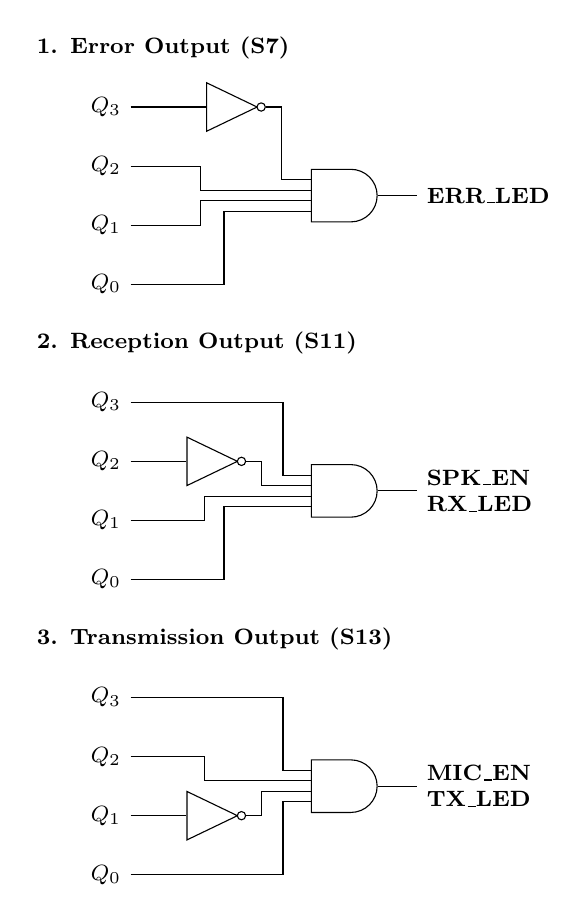
\begin{tikzpicture}[
    circuit logic US,
    small circuit symbols, % Reduced gate size
    every node/.style={font=\footnotesize},
]

% =========================================================
% 1. Error Output (S7)
% =========================================================
\node[anchor=west] at (-1, 3.75) {\textbf{1. Error Output (S7)}};

% The 4-input AND Gate positioned at x=3
\node[and gate, inputs={nnnn}, point right] (AND1) at (3,1.875) {};

% Inputs positioned at x=0 with generous vertical spacing (0.4cm gap)
\node (q3_1) at (0, 3) {$Q_3$};
\node (q2_1) at (0, 2.25) {$Q_2$};
\node (q1_1) at (0, 1.5) {$Q_1$};
\node (q0_1) at (0, 0.75) {$Q_0$};

% Wires & NOT Gate
% Q3 -> NOT -> Input 1
\node[not gate, point right] (NOT1) at (1.5, 3) {}; % NOT gate in the middle (x=1.5)
\draw (q3_1) -- (NOT1.input);
\draw (NOT1.output) -- ++(right:0.2) |- (AND1.input 1);

% Q2 -> Input 2 (Direct wire, bending into input)
\draw (q2_1) -- ++(right:1.2) |- (AND1.input 2);

% Q1 -> Input 3
\draw (q1_1) -- ++(right:1.2) |- (AND1.input 3);

% Q0 -> Input 4
\draw (q0_1) -- ++(right:1.5) |- (AND1.input 4);

% Output Label
\draw (AND1.output) -- ++(0.5,0) node[right] {\textbf{ERR\_LED}};


% =========================================================
% 2. Reception Output (S11)
% =========================================================
\node[anchor=west] at (-1, -0) {\textbf{2. Reception Output (S11)}};

\node[and gate, inputs={nnnn}, point right] (AND2) at (3,-1.875) {};

% Inputs for Circuit 2
\node (q3_2) at (0, -0.75) {$Q_3$};
\node (q2_2) at (0, -1.5) {$Q_2$};
\node (q1_2) at (0, -2.25) {$Q_1$};
\node (q0_2) at (0, -3) {$Q_0$};

% Q3 -> Input 1
\draw (q3_2) -- ++(right:2.25) |- (AND2.input 1);

% Q2 -> NOT -> Input 2
\node[not gate, point right] (NOT2) at (1.25, -1.5) {};
\draw (q2_2) -- (NOT2.input);
\draw (NOT2.output) -- ++(right:0.2) |- (AND2.input 2);

% Q1 -> Input 3
\draw (q1_2) -- ++(right:1.25) |- (AND2.input 3);

% Q0 -> Input 4
\draw (q0_2) -- ++(right:1.5) |- (AND2.input 4);

% Output Label
\draw (AND2.output) -- ++(0.5,0) node[right, align=left] {\textbf{SPK\_EN} \\ \textbf{RX\_LED}};


% =========================================================
% 3. Transmission Output (S13)
% =========================================================
\node[anchor=west] at (-1, -3.75) {\textbf{3. Transmission Output (S13)}};

\node[and gate, inputs={nnnn}, point right] (AND3) at (3,-5.625) {};

% Inputs for Circuit 3
\node (q3_3) at (0, -4.5) {$Q_3$};
\node (q2_3) at (0, -5.25) {$Q_2$};
\node (q1_3) at (0, -6) {$Q_1$};
\node (q0_3) at (0, -6.75) {$Q_0$};

% Q3 -> Input 1
\draw (q3_3) -- ++(right:2.25) |- (AND3.input 1);

% Q2 -> Input 2
\draw (q2_3) -- ++(right:1.25) |- (AND3.input 2);

% Q1 -> NOT -> Input 3
\node[not gate, point right] (NOT3) at (1.25, -6) {};
\draw (q1_3) -- (NOT3.input);
\draw (NOT3.output) -- ++(right:0.2) |- (AND3.input 3);

% Q0 -> Input 4
\draw (q0_3) -- ++(right:2.25) |- (AND3.input 4);

% Output Label
\draw (AND3.output) -- ++(0.5,0) node[right, align=left] {\textbf{MIC\_EN} \\ \textbf{TX\_LED}};

\end{tikzpicture}

\newpage

% 8. Organigramă cu microinstrucțiuni
\section{Implementarea cu microinstrucțiuni variabile}
\subsection{Organigrama pentru implementarea cu microinstrucțiuni}
\begin{figure}[ht!]
    \centering
    \usetikzlibrary{shapes.multipart, arrows, positioning, calc}
    
    % Resize logic: Scale to width, but ensure height doesn't exceed page limits
    \resizebox{\textwidth}{!}{%
    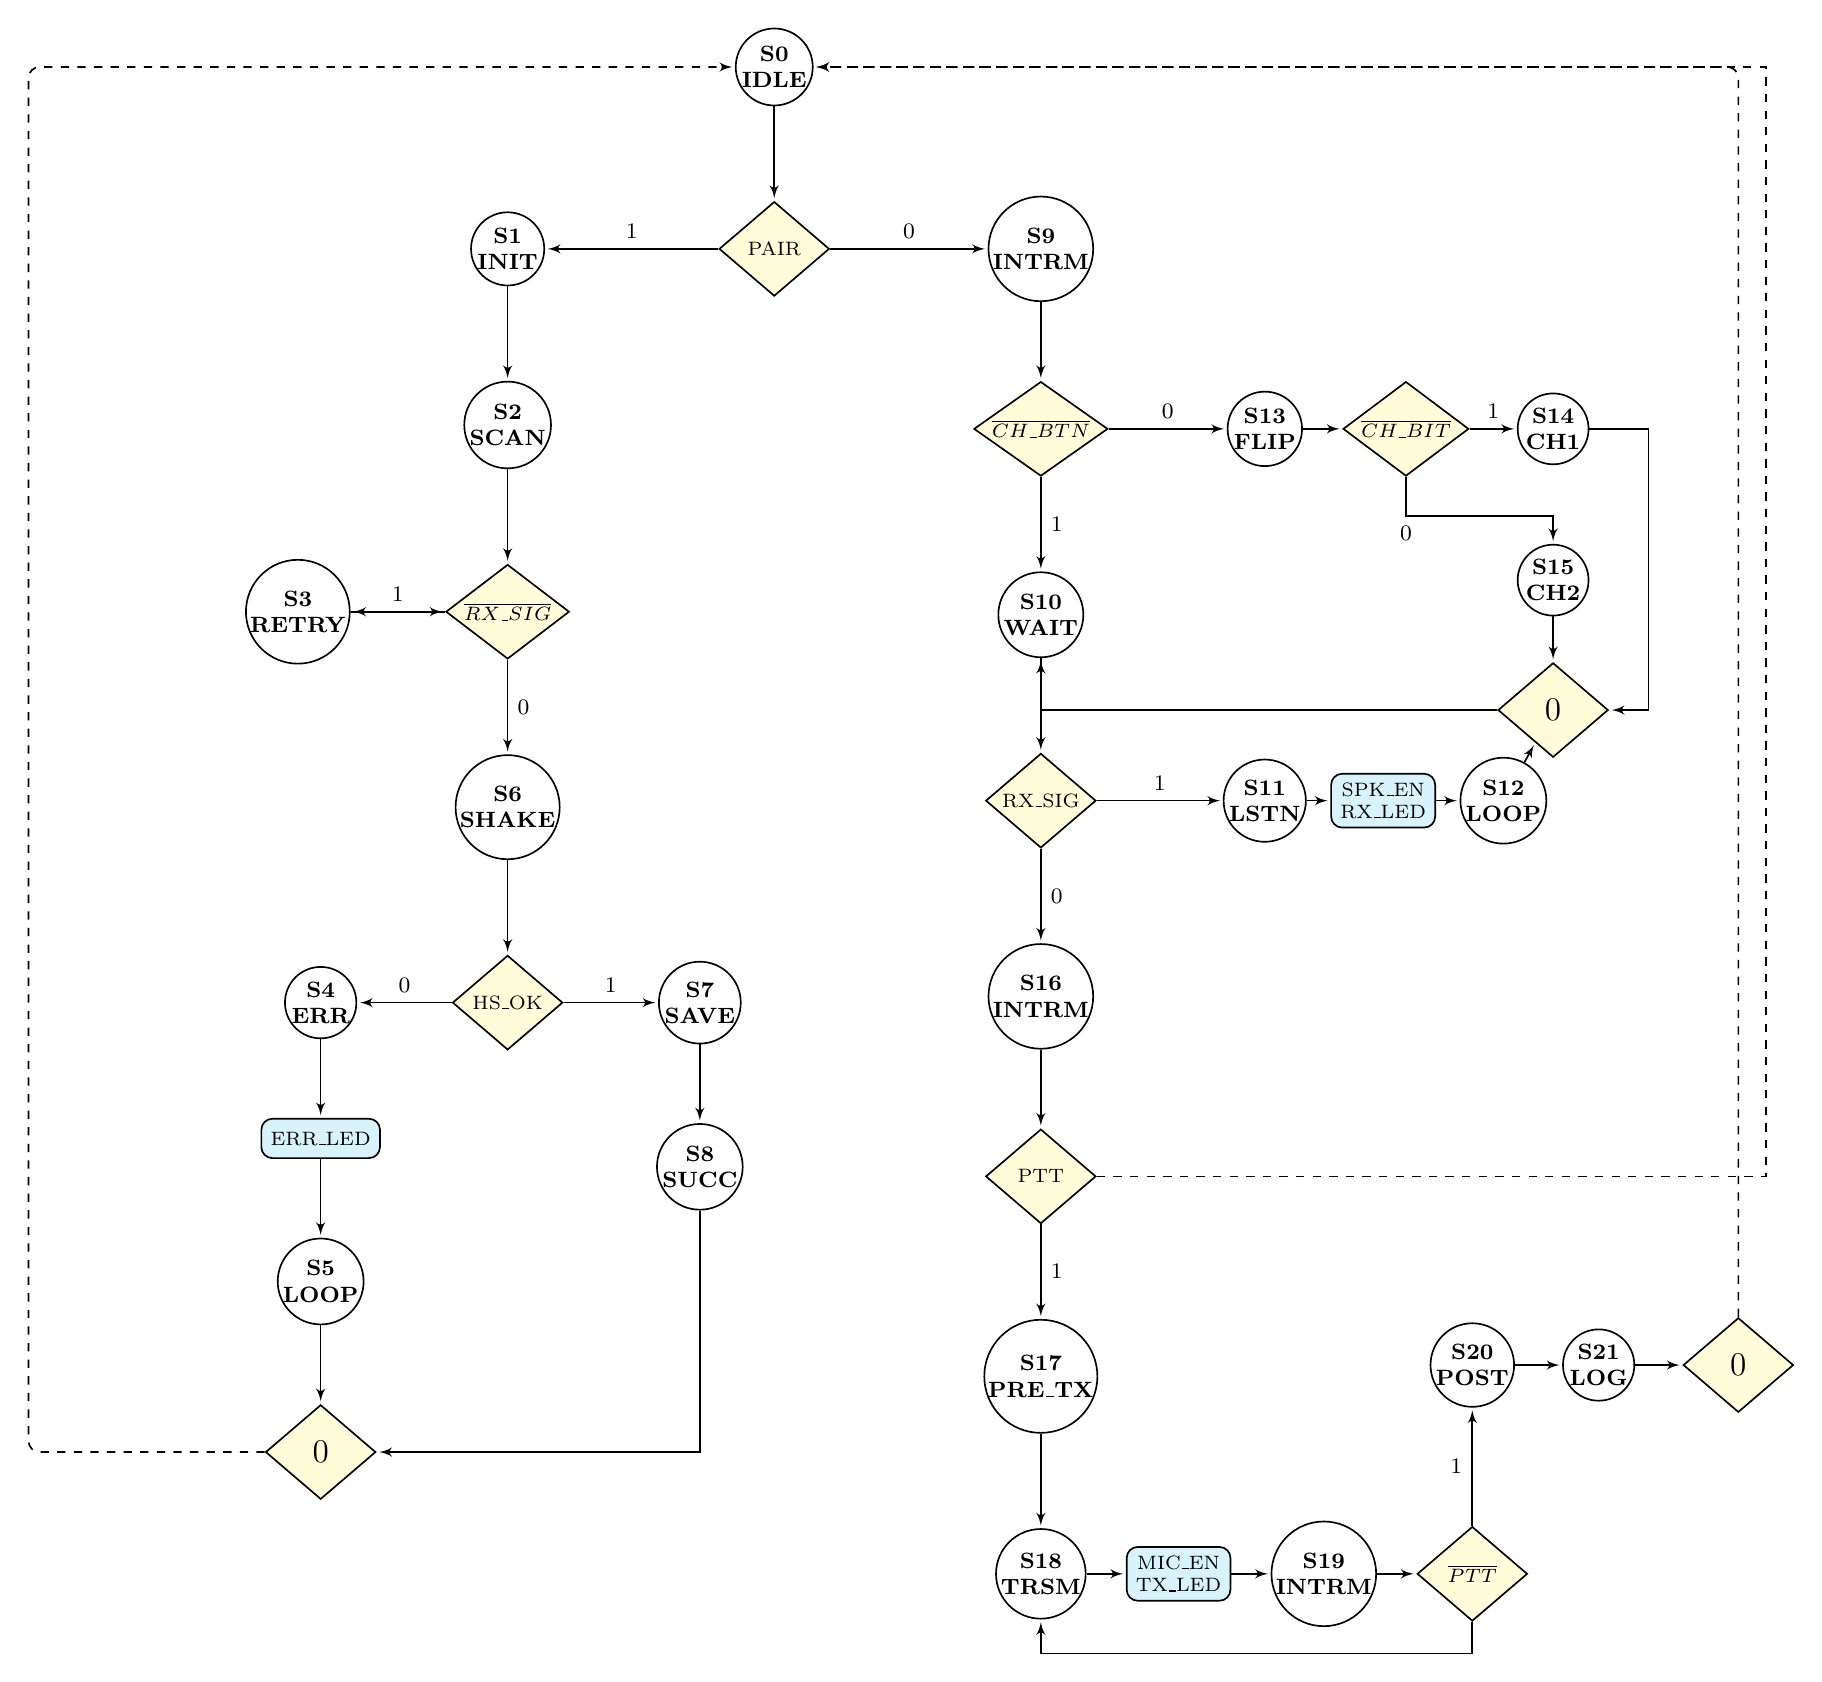
\begin{tikzpicture}[->, >=latex', shorten >=1pt, auto, node distance=1.2cm, semithick, font=\footnotesize]

        % Styles from organigram.tex
        \tikzstyle{state} = [circle, draw, minimum size=0.9cm, align=center, fill=white, font=\footnotesize\bfseries, inner sep=0pt]
        \tikzstyle{moore} = [circle split, draw, minimum size=1.0cm, align=center, fill=cyan!15, font=\footnotesize\bfseries, inner sep=1pt]
        \tikzstyle{decision} = [diamond, draw, aspect=2.0, inner sep=0pt, minimum width=1.4cm, minimum height=1.2cm, align=center, fill=yellow!15, font=\scriptsize]
        \tikzstyle{output} = [rectangle, draw, rounded corners, minimum height=0.5cm, align=center, fill=cyan!15, font=\scriptsize]

        % --- CENTRAL SPINE ---
        % ID 0: S0 IDLE
        \node[state] (S0) {S0\\IDLE};
        
        \node[decision, below=1.2cm of S0] (d_pair) {PAIR};

        % --- LEFT BRANCH (Pairing) ---
        % ID 1: S1 INIT
        \node[state, left=2.2cm of d_pair] (S1) {S1\\INIT};
        
        % ID 2: S2 SCAN
        \node[state, below=1.2cm of S1] (S2) {S2\\SCAN};
        \node[decision, below=1.2cm of S2] (d_rx1) {$\overline{RX\_SIG}$};
        
        % ID 6: S3 RETRY (Source ID 3)
        \node[state, left=1.2cm of d_rx1] (S3) {S3\\RETRY};
        
        % ID 3: S4 SHAKE (Source ID 6)
        \node[state, below=1.2cm of d_rx1] (S6) {S6\\SHAKE};
        \node[decision, below=1.2cm of S6] (d_hs) {HS\_OK};
        
        % ID 7: S7 ERR (Source ID 4)
        \node[state, left=1.2cm of d_hs] (S4) {S4\\ERR};
        \node[output, below=1.0cm of S4] (err_led) {ERR\_LED};
        
        % ID 8: Loop Helper (Source I7 5)
        \node[state, below=1.0cm of err_led] (S5) {S5\\LOOP};
        \node[decision, below=1.0cm of S5] (false_34) {\large{0}};
        
        % ID 4: S5 SAVE (Source ID S7)
        \node[state, right=1.2cm of d_hs] (S7) {S7\\SAVE};
        
        % ID 5: S6 SUCC (Source ID 8)
        \node[state, below=1.0cm of S7] (S8) {S8\\SUCC};

        % --- RIGHT BRANCH (Channel) ---
        % ID 9: Intermediary (Source ID 9)
        \node[state, right=2.0cm of d_pair] (S9) {S9\\INTRM};
        \node[decision, below=1.0cm of S9] (d_inv_ch) {$\overline{CH\_BTN}$};
        
        % ID 13: Channel Flip (Source ID 13)
        \node[state, right=1.5cm of d_inv_ch] (S13) {S13\\FLIP};
        \node[decision, right=0.5cm of S13] (d_inv_bit) {$\overline{CH\_BIT}$};
        
        % ID 14: S8 CH1 (Source ID 14)
        \node[state, right=0.6cm of d_inv_bit] (S14) {S14\\CH1};
        
        % ID 15: S9 CH2 (Source ID 15)
        \node[state, below=1.0cm of S14] (S15) {S15\\CH2};
        
        % Logic ID 85: Always False
        \node[decision, below=2.5cm of S14] (false_85) {\large{0}};

        % --- WAIT & RX BRANCH ---
        % ID 10: S10 WAIT
        \node[state, below=1.2cm of d_inv_ch] (S10) {S10\\WAIT};
        \node[decision, below=1.2cm of S10] (d_rx2) {RX\_SIG};
        
        % ID 11: S11 LSTN
        \node[state, right=1.6cm of d_rx2] (S11) {S11\\LSTN};
        \node[output, right=0.3cm of S11] (spk_led) {SPK\_EN\\RX\_LED};
        
        % ID 12: Loop Helper (Source ID 12)
        \node[state, right=0.3cm of spk_led] (S12) {S12\\LOOP};

        % --- TX BRANCH ---
        % ID 16: Intermediary (Source ID 16)
        \node[state, below=1.2cm of d_rx2] (S16) {S16\\INTRM};
        \node[decision, below=1.0cm of S16] (d_ptt) {PTT};
        
        % ID 17: S12 PRE_TX (Source ID 17)
        \node[state, below=1.2cm of d_ptt] (S17) {S17\\PRE\_TX};
        
        % ID 18: S13 TRSM (Source ID 18)
        \node[state, below=1.2cm of S17] (S18) {S18\\TRSM};
        \node[output, right=0.5cm of S18] (mic_led) {MIC\_EN\\TX\_LED};
        
        % ID 19: Intermediary (Source ID 19)
        \node[state, right=0.5cm of mic_led] (S19) {S19\\INTRM};
        \node[decision, right=0.5cm of S19] (d_inv_ptt) {$\overline{PTT}$};
        
        % ID 20: S14 POST (Source ID 20)
        \node[state, above=1.5cm of d_inv_ptt] (S20) {S20\\POST};
        
        % ID 21: S15 LOG (Source ID 21)
        \node[state, right=0.6cm of S20] (S21) {S21\\LOG};
        \node[decision, right=0.6cm of S21] (false_106) {\large{0}};

        % --- EDGES ---

        % 1. Start
        \path (S0) edge (d_pair);

        % 2. Pairing
        \path (d_pair) edge node[above] {1} (S1);
        \path (S1) edge (S2);
        \path (S2) edge (d_rx1);
        
        % Retry (ID 6)
        \path (d_rx1) edge node[above] {1} (S3);
        \path (S3) edge (d_rx1);
        
        % Shake (ID 3)
        \path (d_rx1) edge node[right] {0} (S6);
        \path (S6) edge (d_hs);
        
        % HS Outcomes
        \path (d_hs) edge node[above] {0} (S4);
        \path (d_hs) edge node[above] {1} (S7);
        
        \path (S7) edge (S8);
        \draw (S8.south) |- (false_34.east);
        
        \path (S4) edge (err_led);
        \path (err_led) edge (S5);
        \path (S5) edge (false_34);
        
        \draw [dashed, rounded corners] (false_34.west) -- ++(-3.0, 0) |- (S0.west);

        % 3. Channel
        \path (d_pair) edge node[above] {0} (S9);
        \path (S9) edge (d_inv_ch);
        
        \path (d_inv_ch) edge node[right] {1} (S10);
        \path (d_inv_ch) edge node[above] {0} (S13);
        
        \path (S13) edge (d_inv_bit);
        \path (d_inv_bit) edge node[above] {1} (S14);
        \draw (d_inv_bit.south) -- ++(0, -0.5) node[below] {0} -| (S15.north);
        
        \draw (S14.east) -- ++(0.75, 0) |- (false_85.east);
        \path (S15) edge (false_85);
        \draw (false_85.west) -| (S10.south);

        % 4. Wait & RX
        \path (S10) edge (d_rx2);
        
        \path (d_rx2) edge node[above] {1} (S11);
        \path (S11) edge (spk_led);
        \path (spk_led) edge (S12);
        \path (S12) edge (false_85);

        % 5. TX
        \path (d_rx2) edge node[right] {0} (S16);
        \path (S16) edge (d_ptt);
        
        \draw [dashed] (d_ptt.east) -- ++(8.5, 0) |- (S0.east);
        \path (d_ptt) edge node[right] {1} (S17);
        \path (S17) edge (S18);
        \path (S18) edge (mic_led);
        \path (mic_led) edge (S19);
        \path (S19) edge (d_inv_ptt);
        
        \draw (d_inv_ptt.south) -- ++(0, -0.4) -| (S18.south);
        \path (d_inv_ptt) edge node[left] {1} (S20);
        \path (S20) edge (S21);
        \path (S21) edge (false_106);
        
        \draw [dashed, rounded corners] (false_106.north) |- (S0.east);

    \end{tikzpicture}
    } % End resizebox
    \caption{Organigrama adaptată pentru implementarea cu microinstrucțiuni}
    \label{fig:drawio_full_translated_spaced_binary}
\end{figure}


% 9. Calculul lungimii microinstrucțiunii
\subsection{Calculul lungimii microinstrucțiunii}
\subsubsection{Date de intrare}
Conform specificațiilor organigramei, parametrii sistemului sunt:
\begin{itemize}
    \item Număr de stări ($N_{stari}$): 22
    \item Număr variabile de intrare ($N_{in}$): 9
    \item Număr variabile de ieșire ($N_{out}$): 5
\end{itemize}

\subsubsection{Dimensionarea câmpurilor}

\begin{enumerate}
    \item \textbf{Câmpul de adresare ($n_{adr}$):}
    Numărul de biți necesari pentru a adresa unic cele 22 de stări se calculează logaritmic:
    \[
    n_{adr} = \log_2(N_{stari}) = \log_2(22)
    \]
    Deoarece $2^4 = 16 < 22 \leq 32 = 2^5$:
    \[
    n_{adr\_necesar} = 5 \text{ biți}
    \]
  Vom alege memoria de tip \textbf{64 x 4} pentru implementarea microinstrucțiunilor așa încât:
    \[
    n_{adr} = \log_2(64) = 6 \text{ biți}
    \]

    \item \textbf{Câmpul condițiilor de intrare ($n_{ci}$):}
    Pentru a selecta una dintre cele 9 variabile de intrare (condiții de test), calculăm:
    \[
    n_{ci} = \log_2(N_{in}) = \log_2(9)
    \]
    Deoarece $2^3 = 8 < 9 \leq 16 = 2^4$:
    \[
    n_{ci} = 4 \text{ biți}
    \]

    Astfel va fi folosit un \textbf{MUX 16:1} pentru schema unității de comandă.

    \item \textbf{Câmpul de ieșire ($n_{out}$):}
    În formatul variabil, pentru instrucțiunile de tip 0 (comandă), biții sunt alocați direct variabilelor de ieșire.
    \[
    n_{out} = 5 \text{ biți}
    \]
\end{enumerate}

\subsubsection{Aplicarea calculului final}

Lungimea microinstrucțiunii este determinată de maximul dintre lungimea necesară pentru instrucțiunile de salt (Tip 1) și cele de comandă (Tip 0), plus bitul de selecție a formatului:

\[
L_{\mu i} = 1 + \max(\underbrace{n_{ci} + n_{adr}}_{\text{Tip 1}}, \underbrace{n_{out}}_{\text{Tip 0}})
\]

Înlocuind valorile calculate:

\[
L_{\mu i} = 1 + \max(4 + 6, 5)
\]
\[
L_{\mu i} = 1 + \max(9, 5)
\]
\[
L_{\mu i} = 1 + 9 = 11 \text{ biți}
\]

\textbf{Concluzie:} Lungimea microinstrucțiunii în format variabil este de \textbf{11 biți}, structurată astfel:
\begin{itemize}
    \item \textbf{Bit 10:} Selector format (1 bit).
    \item \textbf{Biții 9-0 (Tip 1):} 4 biți pentru condiționale + 6 biți pentru adresele stărilor (primul bit pentru adresele stărilor va fi mereu 0, deoarece sunt doar 5 biți de adresă necesari).
    \item \textbf{Biții 9-0 (Tip 0):} 5 biți utilizați pentru Ieșiri (restul de 5 biți fiind neutilizați).
\end{itemize}

  Vom concatena \textbf{3 circuite} de memorie \textbf{64 x 4} pentru implementarea dispozitivului.

%
% TBD:
% % 9. Proiectarea unității de comandă microprogramată
% \section{Proiectarea unității de comandă microprogramată}
% \begin{tikzpicture}[
    >={Stealth}, % Default arrow tip
    % --- Styles ---
    % Main blocks
    block/.style={draw, rectangle, minimum height=1cm, inner sep=5pt, align=center},
    % MUX style
    mux/.style={draw, rectangle, minimum width=3cm, minimum height=8.5cm},
    % Bus style (double lines) with explicit arrow tip
    bus/.style={double, double distance=1.5pt, line width=0.8pt, -{Stealth[length=3mm, width=2mm]}},
    % Simple wire style with filled arrow
    wire/.style={line width=0.8pt, ->},
    % Plain line (no arrow) used for segments before a turn
    line/.style={line width=0.8pt},
    % Logic gates
    logic/.style={draw, logic gate inputs=nn},
    % Node alignment
    every node/.style={align=center}
]

    % 1. TOP MEMORY / INSTRUCTION REGISTER (ROM)
    \node[inner sep=0pt] (rom) {
        \renewcommand{\arraystretch}{1.8}
        \setlength{\tabcolsep}{0pt}
        \begin{tabular}{|>{\centering\arraybackslash}p{1.2cm}|>{\centering\arraybackslash}p{2.8cm}|>{\centering\arraybackslash}p{3.2cm}|}
            \hline
            TIP 1 & \multicolumn{2}{c|}{SEMNALE DE IE\c{S}IRE} \\
            \hline
            TIP 0 & \textcolor{green!60!black}{INPCOD} & \textcolor{red!80!black}{ADR 0} \\
            \hline
        \end{tabular}
    };

    % --- Define Accurate Anchors ---
    \coordinate (tip0_center) at ($(rom.south west) + (0.6, 0)$); 
    \coordinate (inpcod_center) at ($(rom.south west) + (2.6, 0)$); 
    \coordinate (adr0_center) at ($(rom.south west) + (5.6, 0)$); 
    
    % Anchors for right-side connections
    \coordinate (semnale_exit) at ($(rom.north east)!0.5!(rom.east)$); 
    \coordinate (adr0_side_entry) at ($(rom.south east)!0.5!(rom.east)$);    

    % 2. COMPONENT PLACEMENT
    
    % MUX: Positioned directly below INPCOD center
    \node[mux] (mux) at ($(inpcod_center) + (0, -6.5)$) {}; 
    
    % MASCA: To the right of Semnale
    \node[block, right=2.5cm of semnale_exit, anchor=west] (masca) {MASCA};
    \node[right=1.0cm of masca] (out_arrow) {OUT};

    % OR Gate: Positioned relative to MUX
    \node[or gate US, draw, logic gate inputs=nn, rotate=0] (or) at ($(mux.east) + (1.5, 0)$) {};

    % NUM: Positioned to the right of OR gate
    \node[block, minimum width=2cm, minimum height=2.5cm] (num) at ($(or.east) + (2.5, -0)$) {NUM};

    % 3. WIRING

    % --- A. CONTROL LINE (TIP 0) ---
    \coordinate (ctrl_level) at ($(rom.south) + (0, -0.7)$); 
    
    % 1. Drop down from TIP 0
    \draw (tip0_center) -- (tip0_center |- ctrl_level);
    
    % 2. Horizontal run to MASCA center
    \draw[wire] (tip0_center |- ctrl_level) -- (masca.south |- ctrl_level) -| (masca.south);
    
    % 3. Branch to Logic (OR gate input 2) - Shifted LEFT
    \coordinate (logic_split) at ($(or.input 2 |- ctrl_level) - (0.4, 0)$);
    \draw[wire] (logic_split) |- (or.input 2);
    \fill (logic_split) circle (1.5pt); % Connection dot

    % --- B. BUSES ---
    
    % 1. INPCOD -> MUX (Vertical Drop)
    \draw[bus] (inpcod_center) -- (mux.north);
    
    % 2. ADR 0 -> NUM (Route Right then Down)
    \draw[bus] (adr0_center) -- ++(0,-1.5) -| ($(num.north) + (0.5, 0.5)$) -- ($(num.north) + (0.5, 0)$);

    % 3. SEMNALE -> MASCA
    \draw[bus] (semnale_exit) -- (masca.west);
    
    % 4. MASCA -> OUT
    \draw[bus] (masca.east) -- (out_arrow.west);

    % 5. FEEDBACK: NUM -> ADR 0 (Side Entry)
    \draw[bus] (num.east) -- ++(0.5,0) |- (adr0_side_entry);
    
    % --- C. LOGIC CONNECTIONS ---
    
    % MUX Output -> OR Input 1
    \draw[wire] (mux.east) |- (or.input 1);
    
    % OR Output -> NUM UP & Branch to LD
    % 1. Define specific target points
    \coordinate (up_label_pos) at ($(num.north west) + (0.1, -0.3)$);
    \coordinate (num_up_in) at (num.west |- up_label_pos);
    
    % LD Input Bubble location
    \coordinate (ld_in) at ($(num.north west) + (-0.2, -0.9)$);
    \draw[thin] (ld_in) circle (1.5pt); % Bubble
    \coordinate (ld_connect) at ($(ld_in) + (-0.23, 0)$); % Connection point left of bubble
    
    % 2. Draw the main path from OR to UP
    \draw[wire] (or.output) -- ++(0.5, 0) coordinate(split_point) |- (num_up_in);
    
    % 3. Draw the Branch to LD
    \draw[wire] (split_point) -- ++(0, 0.2) node[above left, font=\scriptsize] {CTRL} |- (ld_connect) -- (ld_in);
    \fill (split_point) -- ++(0, 0.35) circle (1.5pt); % Connection dot

    % --- D. CLOCK ---
    \draw[wire] ($(num.south) + (0,-0.8)$) -- (num.south);
    \node[right, font=\scriptsize] at ($(num.south) + (0,-0.6)$) {CEAS};

    % --- E. LABELS & PINS ---
    
    \node[anchor=east] at ($(mux.east) + (-0.5, 0.5)$) {\large MUX};
    \node[anchor=east] at ($(mux.east) + (-0.55, 0)$) {16 : 1};
    \node at ($(mux.south) + (0,-0.25)$) {$\overline{EN}$};

    % MUX Input Pins with Arrows
    % Note: Underscores in labels must be escaped (e.g., RX\_SIG)
    \foreach \i/\lbl/\inv/\bin [count=\y from 0] in {
        0/PAIR/0/0000, 
        1/RX\_SIG/0/0001, 
        2/RX\_SIG/1/0010, 
        3/CH\_BTN/1/0011,
        4/CH\_BIT/1/0100, 
        5/PTT/0/0101, 
        6/PTT/1/0110, 
        7/HS\_OK/0/0111,
        8/{*}/0/{......}, 
        9/{0}/0/1111%
    } {
        \coordinate (pin\y) at ($(mux.north west)!0.1 + 0.09*\y!(mux.south west)$);
        \node[anchor=west, font=\scriptsize] at ($(pin\y) + (0.1,0)$) {\bin};
        
        \ifnum\inv=1
            \draw[thin] ($(pin\y) + (-0.3,0)$) circle (2pt);
            \draw (pin\y) -- ($(pin\y) + (-0.23,0)$); 
            \draw[wire] ($(pin\y) + (-1.2,0)$) -- ($(pin\y) + (-0.37,0)$);
            \node[anchor=east] at ($(pin\y) + (-1.2,0)$) {\lbl};
        \else
            \draw[wire] ($(pin\y) + (-1.2,0)$) -- (pin\y);
            \node[anchor=east] at ($(pin\y) + (-1.2,0)$) {\lbl};
        \fi
    }

    % NUM Labels
    \node[anchor=west, font=\scriptsize] at ($(num.north west) + (0, -0.3)$) {UP};
    \node[anchor=west, font=\scriptsize] at ($(num.north west) + (0,-0.9)$) {LD};

\end{tikzpicture}

%
% % 10. Alegerea componentelor digitale
% \section{Alegerea componentelor digitale}
% \subsubsection{Memorie}
Pentru implementarea memoriei de comandă, s-au luat în considerare următoarele cerințe:
\begin{itemize}
    \item \textbf{Lungimea microinstrucțiunilor:} 10 biți (necesar $\ge 8$).
    \item \textbf{Număr de stări:} 22 (necesar $\ge 16$).
\end{itemize}

\textbf{Soluția aleasă:}
S-a optat pentru utilizarea a 3 memorii de 4 biți și 64 cuvinte, model \textbf{CAT22C10} (SRAM/EEPROM), conectate în paralel.
\begin{itemize}
    \item Deși modelul 74HC7403 (Phillips) a fost considerat, CAT22C10 este utilizat mai frecvent.
    \item Prin legarea în paralel, se obțin disponibili 12 biți, dintre care 2 vor rămâne neutilizați.
\end{itemize}

\subsubsection{Multiplexare}
Gestionarea tranzițiilor de stare necesită selectarea sursei pentru adresa următoare.
\begin{itemize}
    \item \textbf{Cerințe:} Sunt necesare 16 intrări (pentru a acomoda cele 9 inputuri de sistem plus logica internă) și 4 biți de selecție.
    \item \textbf{Soluția aleasă:} Un multiplexor 16-la-1 din familia 54150, specific modelul \textbf{SN54150}.
\end{itemize}

\subsubsection{Numărătoare}
Pentru secvențierea stărilor, este necesar un sistem de numărare capabil să adreseze cele 22 de stări.
\begin{itemize}
    \item \textbf{Adresare:} 22 de stări necesită adrese de 5 biți, deoarece $2^4 = 16 < 22 < 2^5 = 32$.
    \item \textbf{Soluția aleasă:} Două numărătoare de 4 biți conectate în cascadă. S-a decis utilizarea cipului \textbf{SN54192} (în detrimentul 74HC161) datorită familiarității.
    \item \textbf{Conexiune:} Pinul de \textit{Carry} al numărătorului de biți mai puțin semnificativi trebuie conectat la pinul \textit{Load/Up} al numărătorului mai semnificativ.
\end{itemize}

\subsubsection{Masca și Porțile Logice}
Logica de control și mascare necesită următoarele componente discrete:
\begin{itemize}
    \item \textbf{Porți AND:} Sunt necesare 5 porți (una pentru fiecare output). Se vor folosi 2 cipuri \textbf{74HC08} (care oferă un total de 8 porți).
    \item \textbf{Invertor:} Este necesar un invertor pentru intrările multiplexorului, asigurat de un cip \textbf{74HC04}.
    \item \textbf{Porți OR:} Este necesar un cip \textbf{74HC32} pentru a decide logica dintre incrementarea numărătorului (+1) sau încărcarea adresei de salt (ADR0).
\end{itemize}

\subsubsection{Detalii Tehnice și Pinout}

Mai jos sunt detaliile pinilor pentru componentele principale identificate în documentație:

\begin{table}[h]
\centering
\begin{tabular}{|l|l|l|}
\hline
\textbf{Componentă} & \textbf{Pin} & \textbf{Funcție/Descriere} \\ \hline
\textbf{CAT22C10} & 8 & $V_{SS}$ (GND) \\
(Memorie) & 18 & $V_{CC}$ \\
 & 1-7 & Adrese ($A_0 - A_5$) și NC \\
 & 11 & WE (Write Enable) \\ \hline
\textbf{SN54150} & 24 & $V_{CC}$ \\
(Multiplexor) & 12 & GND \\
 & 11, 13-15 & Selecție ($S_0 - S_3$) \\
 & 10 & Output Inverted ($\bar{W}$) \\ \hline
\textbf{SN54192} & 16 & $V_{CC}$ \\
(Counter) & 8 & GND \\
 & 5 & UP (Count Up) \\
 & 4 & DOWN (Count Down) \\
 & 11 & $\overline{LOAD}$ \\ \hline
\end{tabular}
\caption{Selecție pini relevanți}
\end{table}

%
% % 11. Completarea memoriei de microprogram
% \section{Completarea memoriei de microprogram}
% \begin{table}[h]
\centering
\renewcommand{\arraystretch}{1.2}
\begin{tabular}{|c|c|c|c|c|l|}
\hline
\textbf{Stare} & \textbf{ID} & \textbf{TIP 1/0} & \textbf{INPCOD} & \textbf{ADR0} & \textbf{Nume} \\
\hline
$S_{0}$ & \texttt{00000} & \texttt{0} & \texttt{000000} & \texttt{1001} & IDLE \\
\hline
$S_{1}$ & \texttt{00001} & \texttt{1} & \texttt{100000} & \texttt{****} & INIT \\
\hline
$S_{2}$ & \texttt{00010} & \texttt{0} & \texttt{000100} & \texttt{0110} & SCAN \\
\hline
$S_{3}$ & \texttt{00011} & \texttt{0} & \texttt{000100} & \texttt{0110} & RETRY \\
\hline
$S_{4}$ & \texttt{00100} & \texttt{1} & \texttt{110000} & \texttt{****} & ERROR \\
\hline
$S_{5}$ & \texttt{00101} & \texttt{0} & \texttt{011110} & \texttt{0000} & LOOP \\
\hline
$S_{6}$ & \texttt{00110} & \texttt{0} & \texttt{001110} & \texttt{0100} & SHAKE \\
\hline
$S_{7}$ & \texttt{00111} & \texttt{1} & \texttt{100000} & \texttt{****} & SAVE \\
\hline
$S_{8}$ & \texttt{01000} & \texttt{0} & \texttt{011110} & \texttt{0000} & SUCCESS \\
\hline
$S_{9}$ & \texttt{01001} & \texttt{0} & \texttt{000110} & \texttt{1101} & INTER \\
\hline
$S_{10}$ & \texttt{01010} & \texttt{0} & \texttt{000011} & \texttt{0000} & WAIT \\
\hline
$S_{11}$ & \texttt{01011} & \texttt{1} & \texttt{101010} & \texttt{****} & LISTEN \\
\hline
$S_{12}$ & \texttt{01100} & \texttt{0} & \texttt{011110} & \texttt{1010} & LOOP \\
\hline
$S_{13}$ & \texttt{01101} & \texttt{0} & \texttt{001000} & \texttt{1111} & FLIP \\
\hline
$S_{14}$ & \texttt{01110} & \texttt{0} & \texttt{011110} & \texttt{1010} & CH1 \\
\hline
$S_{15}$ & \texttt{01111} & \texttt{0} & \texttt{011110} & \texttt{1010} & CH2 \\
\hline
$S_{16}$ & \texttt{10000} & \texttt{0} & \texttt{001010} & \texttt{0000} & INTER \\
\hline
$S_{17}$ & \texttt{10001} & \texttt{1} & \texttt{100000} & \texttt{****} & PRE\_TX \\
\hline
$S_{18}$ & \texttt{10010} & \texttt{1} & \texttt{100101} & \texttt{****} & TRANSMIT \\
\hline
$S_{19}$ & \texttt{10011} & \texttt{0} & \texttt{001101} & \texttt{0010} & INTER \\
\hline
$S_{20}$ & \texttt{10100} & \texttt{1} & \texttt{100000} & \texttt{****} & POST \\
\hline
$S_{21}$ & \texttt{10101} & \texttt{0} & \texttt{011110} & \texttt{0000} & LOG \\
\hline
\end{tabular}
\caption{Conținutul memoriei de microprogram}
\end{table}


\end{document}
